\documentclass{standalone}
\usepackage{chez}

\begin{document}
\chapter{November 09, 2020}

Today is the take-home midterm, so we will do some examples
for more relaxing content.

\section{Calculating cup products by brute force}
Let's calculate \(H^*(K; \FF_2)\), where \(K\) is the Klein bottle,
along with the ring structure.
We have the following semisimplicial structure:
\begin{center}
  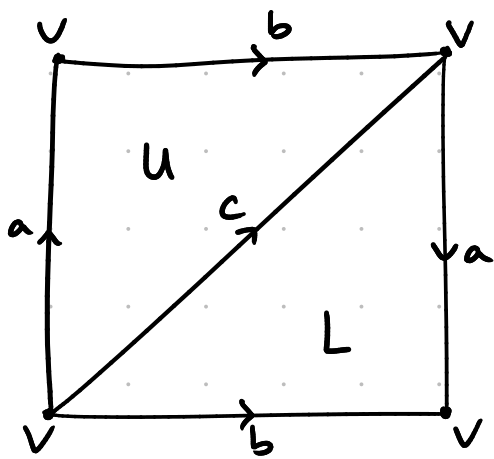
\includegraphics[width=0.2\textwidth]{18_905-201109-1.png}
\end{center}
The chain complex \(S_*(K)\) is
\[
  \begin{tikzcd}
    \cdots \ar[r] &
      \ZZ\fgen{U, L} \ar[r] &
      \ZZ\fgen{a, b, c} \ar[r] &
      \ZZ\fgen{v} \ar[r] &
      0 \ar[r] &
      \cdots
  \end{tikzcd}
\]
To compute the cochain complex \(S^*(K; \FF_2)\),
we have that \(S^0(K; \FF_2) = \ul\Hom(\ZZ\fgen{v}, \FF_2)\).
In particular, a function in \(S^0(K; \FF_2)\) is determined by
where it maps each generator in \(S_0(K)\),
so \(S^0(K; \FF_2) = \FF_2\fgen{\delta_v}\),
where \(\delta_v \colon \ZZ\fgen{v} \to \FF_2\) is
the element corresponding to the generator in the dual vector space.
Similarly, \(S^1(K; \FF_2) = \FF_2\fgen{\delta_a, \delta_b, \delta_c}\), and
\(S^2(K; \FF_2) = \FF_2\fgen{\delta_U, \delta_L}\).
This gives the entire cochain complex \(S^*(K; \FF_2)\):
\[
  \begin{tikzcd}
    \cdots \ar[r] &
      \FF_2\fgen{\delta_v} \ar[r, "\partial"] &
      \FF_2\fgen{\delta_a, \delta_b, \delta_c} \ar[r, "\partial"] &
      \FF_2\fgen{\delta_U, \delta_L} \ar[r] &
      0 \ar[r] &
      \cdots
  \end{tikzcd}
\]

Let's determine what the coboundary morphisms do.
We can use the universal coefficient theorem,
but we will do it manually here.
To calculate \(\partial(\delta_v)\),
note that it is the map \(\ZZ\fgen{a, b, c} \to \FF_2\)
obtained by composing \(\delta_v\) with the boundary map
\(\partial\) in the regular chain complex.
However, note that \(\partial\) maps \(a, b, c \mapsto 0\), so
\(\partial(\delta_v)(a) = \partial(\delta_v)(b) = \partial(\delta_v)(c) = 0\),
and \(\partial(\delta_v) = 0\).

Now let's calculate \(\partial(\delta_a)\),
                    \(\partial(\delta_b)\), and.
In the regular chain complex,
we have \(U \mapsto a + b - c\) and \(L \mapsto c + a - b\).
This gives
\begin{align*}
  \partial(\delta_a)(U) &= \delta_a(a + b - c) = 1 \\
  \partial(\delta_a)(L) &= \delta_a(c + a - b) = 1 \\
  \partial(\delta_b)(U) &= \delta_b(a + b - c) = 1 \\
  \partial(\delta_b)(L) &= \delta_b(c + a - b) = -1 = 1 \\
  \partial(\delta_c)(U) &= \delta_c(a + b - c) = -1 = 1 \\
  \partial(\delta_c)(L) &= \delta_c(c + a - b) = 1.
\end{align*}
Therefore, \(\partial\) maps
\(\delta_a, \delta_b, \delta_c \mapsto \delta_U, \delta_L\).
This gives the cochain complex
\[
  \begin{tikzcd}[row sep=0]
    \cdots \ar[r] &
      \FF_2\fgen{\delta_v} \ar[r, "\partial = 0"] &
      \FF_2\fgen{\delta_a, \delta_b, \delta_c} \ar[r, "\partial"] &
      \FF_2\fgen{\delta_U, \delta_L} \ar[r] &
      0 \ar[r] &
      \cdots \\
    & & \delta_a \ar[r, mapsto] & \delta_U + \delta_L \\[-0.5ex]
    & & \delta_b \ar[r, mapsto] & \delta_U + \delta_L \\[-0.5ex]
    & & \delta_c \ar[r, mapsto] & \delta_U + \delta_L
  \end{tikzcd}
\]

We can then calculate the cohomology:
\begin{align*}
  H^0(K; \FF_2) &\iso \FF_2\fgen{\delta_v} \\
  H^1(K; \FF_2) &\iso \ker \partial
                 \iso \FF_2\fgen{\delta_a + \delta_b, \delta_b + \delta_c} \\
  H^2(K; \FF_2) &= \frac{\FF_2\fgen{\delta_U, \delta_L}}{\delta_U + \delta_L}
                 \iso \FF_2\fgen{k}.
\end{align*}
Let \(\alpha \coloneqq \delta_a + \delta_b\),
    \(\beta \coloneqq \delta_b + \delta_c\), and
    \(k \coloneqq \delta_U\).

We can also compute the cup product structure.
For instance, we can calculate
\(\alpha^2 = (\delta_a + \delta_b)(\delta_a + \delta_b) \in H^2(K; \FF_2)\).
To do this, we determine how it acts on \(U\) and \(L\).
\begin{center}
  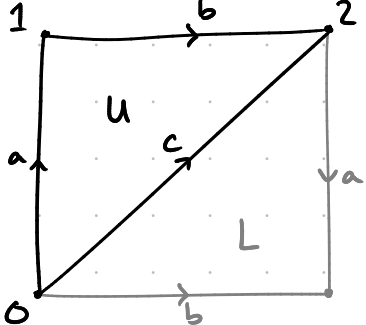
\includegraphics[width=0.2\textwidth]{18_905-201109-2.png}
  \qquad
  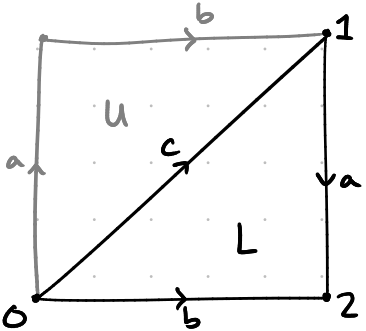
\includegraphics[width=0.2\textwidth]{18_905-201109-3.png}
\end{center}
The front \(1\)-face of \(U\) is \(a\) and
the back \(1\)-face of \(U\) is \(b\).
Therefore,
\[
  \parens[\big]{(\delta_a + \delta_b)(\delta_a + \delta_b)}(U)
    = \parens[\big]{(\delta_a + \delta_b)(a)}
      \parens[\big]{(\delta_a + \delta_b)(b)}
    = (1 + 0)(0 + 1) = 1.
\]
Similarly, the front \(1\)-face of \(U\) is \(a\) and
           the back \(1\)-face of \(U\) is \(b\), so
\[
  \parens[\big]{(\delta_a + \delta_b)(\delta_a + \delta_b)}(L)
    = \parens[\big]{(\delta_a + \delta_b)(c)}
      \parens[\big]{(\delta_a + \delta_b)(a)}
    = (0 + 0)(1 + 0) = 0.
\]
Therefore,
\(\alpha^2 = (\delta_a + \delta_b)(\delta_a + \delta_b) = \delta_U = k\).

Similarly, we can calculate
\begin{align*}
  \parens[\big]{(\delta_b + \delta_c)(\delta_b + \delta_c)}(U)
    &= \parens[\big]{(\delta_b + \delta_c)(a)}
       \parens[\big]{(\delta_b + \delta_c)(b)}
    = (0 + 0)(1 + 0) = 0 \\
  \parens[\big]{(\delta_b + \delta_c)(\delta_b + \delta_c)}(L)
    &= \parens[\big]{(\delta_b + \delta_c)(c)}
       \parens[\big]{(\delta_b + \delta_c)(a)}
    = (0 + 1)(0 + 0) = 0 \\
  \parens[\big]{(\delta_a + \delta_b)(\delta_b + \delta_c)}(U)
    &= \parens[\big]{(\delta_a + \delta_b)(a)}
       \parens[\big]{(\delta_b + \delta_c)(b)}
    = (1 + 0)(1 + 0) = 1 \\
  \parens[\big]{(\delta_a + \delta_b)(\delta_b + \delta_c)}(L)
    &= \parens[\big]{(\delta_a + \delta_b)(c)}
       \parens[\big]{(\delta_b + \delta_c)(a)}
    = (0 + 0)(0 + 0) = 0,
\end{align*}
which means \(\beta^2 = 0\) and \(\alpha\beta = k\).

Therefore, if we consider
\[
  H^*(K; \FF_2)
    \iso \underbracket{\FF_2\fgen{1}}_{\deg 0} \oplus
         \underbracket{\FF_2\fgen{\alpha}
                \oplus \FF_2\fgen{\beta}}_{\deg 1} \oplus
         \underbracket{\FF_2\fgen{k}}_{\deg 2},
\]
we have \(\alpha^2 = \alpha \beta = k\),
        \(\beta^2 = 0\), and
        \(k\alpha = k \beta = k^2 = 0\).
 






\end{document}
